\documentclass[12pt]{article}

%Preamble

\usepackage{amsmath}
\usepackage{amssymb}
\usepackage{amsthm}
\usepackage{amsrefs}
\usepackage{amsfonts}
%\usepackage{dsfont}
\usepackage{mathrsfs}
\usepackage{mathtools}
%\usepackage{stmaryrd}
%\usepackage[all]{xy}
\usepackage{enumerate}
\usepackage[shortlabels]{enumitem}
\usepackage{verbatim} %% includes comment environment
\usepackage{hyperref}
\usepackage[capitalize]{cleveref}
\crefformat{equation}{~(#2#1#3)}
\usepackage{caption, subcaption}
\usepackage{graphicx}
\graphicspath{{figures/}}
\usepackage{fullpage} %%smaller margins
\usepackage[all,arc]{xy}
\usepackage{mathrsfs}

%% Sectioning, Header / Footer, ToC
\usepackage{titlesec}
\usepackage{fancyhdr}
\usepackage{tocloft}


%% Optional Code Snippets

%\usepackage{minted} %Render Code.
%% Must add (% !TEX option = --shell-escape) to top of page.
%\usemintedstyle{colorful}

\hypersetup{
    linktoc=all,     %set to all if you want both sections and subsections linked
}

\newcommand{\bbF}{\mathbb{F}}
\newcommand{\bbN}{\mathbb{N}}
\newcommand{\bbQ}{\mathbb{Q}}
\newcommand{\bbR}{\mathbb{R}}
\newcommand{\bbZ}{\mathbb{Z}}
\newcommand{\bbC}{\mathbb{C}}
\newcommand{\calF}{\mathcal{F}}
\newcommand{\Prob}{\mathbb{P}}
\newcommand{\Expect}{\mathbb{E}}
\newcommand{\Var}{\mathbb{V}}
\newcommand{\Cov}{\text{Cov}}

\newcommand{\abs}[1]{ \left| #1 \right| }
\newcommand{\diff}[2]{\frac{d #1}{d #2}}
\newcommand{\pdiff}[2]{\frac{\partial#1}{\partial #2}}
\newcommand{\infsum}[1]{\sum_{#1}^{\infty}}
\newcommand{\norm}[1]{ \left|\left| #1 \right|\right| }
\newcommand{\eval}[1]{ \left. #1 \right| }

\renewcommand{\phi}{\varphi}

% Indicator Function
\DeclareSymbolFont{bbold}{U}{bbold}{m}{n}
\DeclareSymbolFontAlphabet{\mathbbold}{bbold}
\newcommand{\ind}{\mathbbold{1}}

%--------Theorem Environments--------
%theoremstyle{plain} --- default
\newtheorem{thm}{Theorem}[section]
\newtheorem{cor}[thm]{Corollary}
\newtheorem{prop}[thm]{Proposition}
\newtheorem{lem}[thm]{Lemma}
\newtheorem{conj}[thm]{Conjecture}
\newtheorem{quest}[thm]{Question}

\theoremstyle{definition}
\newtheorem{defn}[thm]{Definition}
\newtheorem{defns}[thm]{Definitions}
\newtheorem{con}[thm]{Construction}
\newtheorem{exmp}[thm]{Example}
\newtheorem{exmps}[thm]{Examples}
\newtheorem{notn}[thm]{Notation}
\newtheorem{notns}[thm]{Notations}
\newtheorem{addm}[thm]{Addendum}
\newtheorem{exer}[thm]{Exercise}

\theoremstyle{remark}
\newtheorem{rem}[thm]{Remark}
\newtheorem{rems}[thm]{Remarks}
\newtheorem{warn}[thm]{Warning}
\newtheorem{sch}[thm]{Scholium}

\numberwithin{equation}{section}

\bibliographystyle{plain}

%% Sectioning Aesthetics
\titleformat{\section}
{\normalfont\Large\bfseries}{\thesection.}{1em}{}
\titleformat{\subsection}
{\normalfont\Large\bfseries}{\thesubsection}{1em}{}
\titleformat{\subsubsection}
{\normalfont\normalsize\bfseries}{\thesubsubsection}{1em}{}
\titleformat{\paragraph}[runin]
{\normalfont\normalsize\bfseries}{\theparagraph}{1em}{}
\titleformat{\subparagraph}[runin]
{\normalfont\normalsize\bfseries}{\thesubparagraph}{1em}{}


%% Header Aesthetics
\pagestyle{fancy}

\setlength{\headheight}{16pt}
\setlength{\headsep}{0.3in}
\renewcommand{\headrulewidth}{0.4pt}
\renewcommand{\footrulewidth}{0.4pt}
\renewcommand{\contentsname}{\hfill\bfseries\Large Table of Contents\hfill}
\renewcommand{\sectionmark}[1]{\markright{ #1}}

\lhead{\textbf{}} % controls the left corner of the header
%\chead{\fancyplain{}{\rightmark }}
 % controls the center of the header / adds section # to top
\rhead[]{Marlin Figgins} % controls the right corner of the header
\lfoot{Last updated: \today} % controls the left corner of the footer
\cfoot{} % controls the center of the footer
\rfoot{Page~\thepage} % controls the right corner of the footer

\title{\bfseries\huge{AMATH 561A: Probability and Random Processes}\vspace{-1ex}} \author{\href{marlinfiggins@gmail.com}{\Large{Marlin Figgins}}\vspace{-2ex}}
\date{\large{Oct. 1, 2020}}

\begin{document}

\maketitle

	\section*{\hfill Introduction \hfill}

  This is a collection of my notes taken during AMATH 561A during fall quarter 2020 at the University of Washington.

  \thispagestyle{empty}

  %% Table of Contents Page/
  \newpage
  \tableofcontents
  \thispagestyle{empty}
  \newpage

  %% Set first page after ToC
  \setcounter{page}{1}

  %% Start here.

  \section{Probability Spaces and Random Variables}%
  \label{sec:probability_spaces_and_random_variables}
  %TODO: Port over some of old notes / blog post figures introducing the study of probability.

  % We'll begin with a slightly informal definition of a probability space. 

  \begin{defn}[Probability Space: Version A]
    A \emph{probability space} is a triple $(\Omega, \calF, \Prob)$ where $\Omega$ is the \emph{sample space} or the space of possible outcomes, $\calF$ is the set of events which are subsets of $\Omega$ and $\Prob \colon \calF \to [0,1]$ is a probability measure that assigns probabilities to events.
 \end{defn} 

 \begin{exmp}[Rolling a fair standard die]
 In this case, we have six possible outcomes as our die is six-sided. Therefore, our sample space is 

 \begin{equation}
   \Omega = \{ 1, 2, 3, 4, 5, 6 \}.
 \end{equation}

 The set of events in this case are all possible subsets of $\Omega$ i.e. the power set $\mathcal{P}(\Omega)$. Finally, since we specificed that the die is fair, each outcome is equally likely, so our probability measure $\Prob$ is uniform over $\Omega$. Therefore, our probability of a given event is just the fraction of our possible out comes which are in the event.

 \begin{equation}
 \Prob(A) = \frac{\abs{A}}{\abs{\Omega}} = \frac{\abs{A}}{6} \text{ for all  } A \in \calF.
 \end{equation}

 For example, we would say that the probability of rolling an even number would be given by

 \begin{equation}
   \Prob(\{ 2, 4, 6 \}) = \frac{3}{6} = 0.5.
 \end{equation}
 \end{exmp}

 In this example, it is simple enough to use all possible subets are our set of events, but as we attempt to deal with more complicated probability spaces, we'll need to develop a more rigorous notion of what constitutes an event, so that our probability measures will have certain properties of interest. This idea is formalized by the $\sigma$-algebra.

 \begin{defn}[$\sigma$-algebra]
   A non-empty collection of subsets of $\Omega$ is a \emph{$\sigma$-algebra} of $\Omega$ if it satistifies the following:

 \begin{enumerate}[(i)]
   \item For each event $A\in \calF$, then its complement $A^c\in \calF$
   \item If we have a countable sequence of sets $A_i \in \calF$, then their union $\bigcup_i A_i \in \calF$.
 \end{enumerate}

 These two conditions form the statement that a $\sigma$-algebra is closed under complements and countable unions.
 \end{defn}

 \begin{prop}
 The definition of the $\sigma$-algebra implies that $\sigma$-algebras are also closed under countable intersection because
 \begin{equation}
   \bigcap_i A_i = \left( \bigcup_i A_i^c \right)^c.
 \end{equation}
 \end{prop}

Minimally, we know that a $\sigma$-algebra must contain the empty set and the space on which it lives. 

\begin{exer}
   Show that any $\sigma$-algebra of $\Omega$ contains both the entire space $\Omega$ and the empty set.
\end{exer}

This formalizes the notion of events and combinations of events espressed earlier. Now, we'll develop a formal notion of probabiltiy usinng measure theory.

%TODO: Clean this up and perhaps limit to probability measures.
 When we have a probability space $\Omega$ and a $\sigma$-algebra $\calF$ on $\Omega$, we can define a measure on the space $(\Omega, \calF)$. \emph{Describe what a measure is intuitively.}

 \begin{defn}[Measure]
   A \emph{measure} is a function $\mu: \calF \to [0, \infty)$ which satisfies:
   \begin{enumerate}[(i)]
     \item $\mu(A) \geq \mu(\emptyset) = 0$ for all $A\in\calF$
     \item if $A_i \in F$ is a countable sequence of disjoint sets, then 
       \begin{equation}
         \mu\left(\bigcup_i A_i \right) = \sum_i \mu(A_i).
       \end{equation}
   \end{enumerate}
   In the case that $\mu(\Omega)$, we will call $\mu$ a \emph{probability measure} and denote it as $\Prob$.
 \end{defn}

 \begin{figure}[ht]
   \centering
   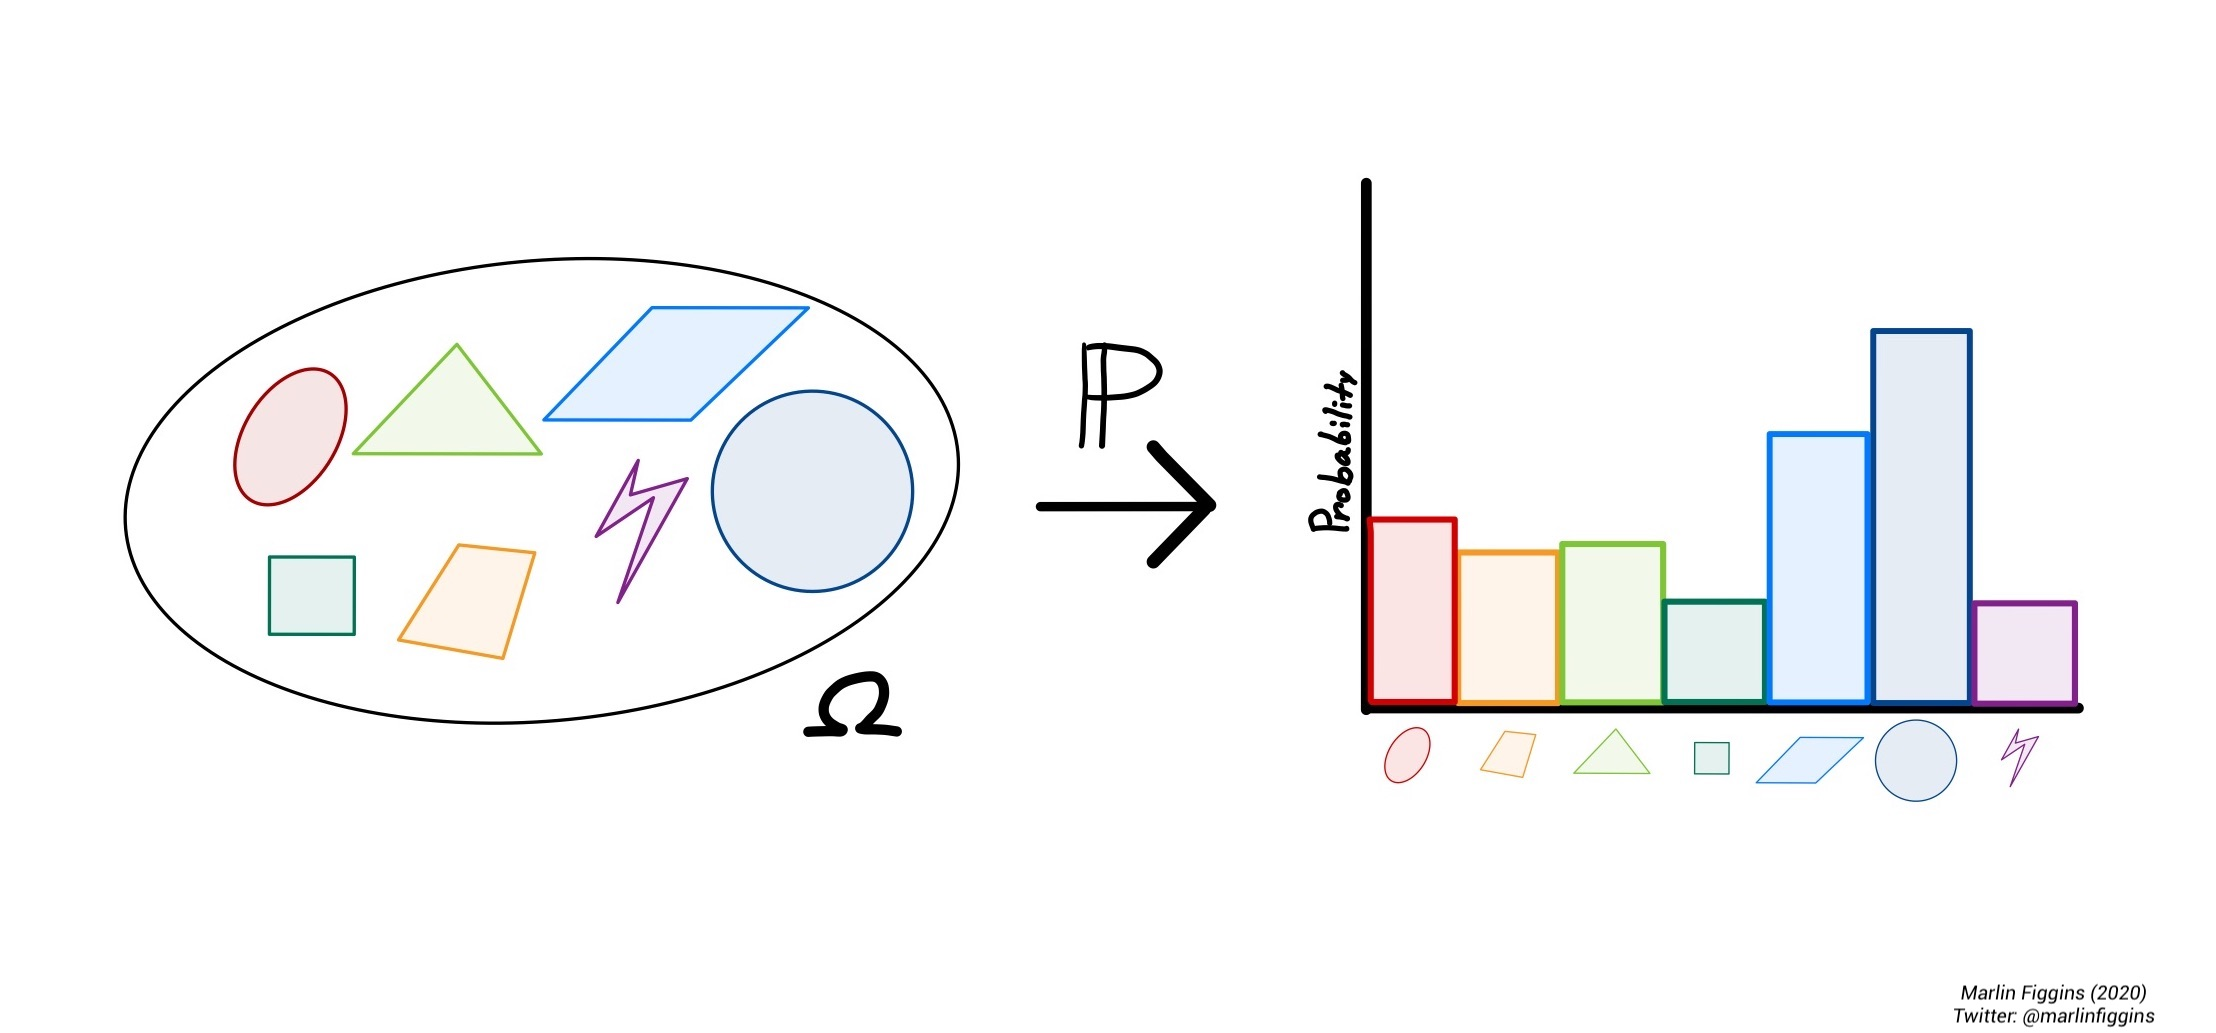
\includegraphics[width=0.9\linewidth]{intro-to-prob-measure.jpg}
   \caption{A probability measure $\Prob$ takes measurable subsets $E\in \calF$ to a numerical value in $[0,1]$.}%
   \label{fig:intro-to-prob-measure}
 \end{figure}

 Our definition of measure allows us to ensure that our notion of probabilty satisifies some of the intuitive properties one might expect of probabilities.

 \begin{thm}[Properties of measure]\leavevmode
   \begin{enumerate}[(i)]
     \item \emph{Monotonicity.} If $A\subset B$, then $\mu(A) \leq  \mu(B)$.
   \item \emph{Subadditivity.} If $A\subset \bigcup_{j\in\bbN} A_j$, then 
        \begin{equation}
        \mu(A) \leq \sum_{j\in\bbN} \mu(A_m).
        \end{equation}
 \end{enumerate}
 \end{thm}

 \begin{proof}[Proof of monotonicity]
   Finish proof. 
 \end{proof}

 \begin{proof}[Proof of subadditivity]
  Finish proof. 
 \end{proof}
 
 \begin{figure}[ht]
   \centering
   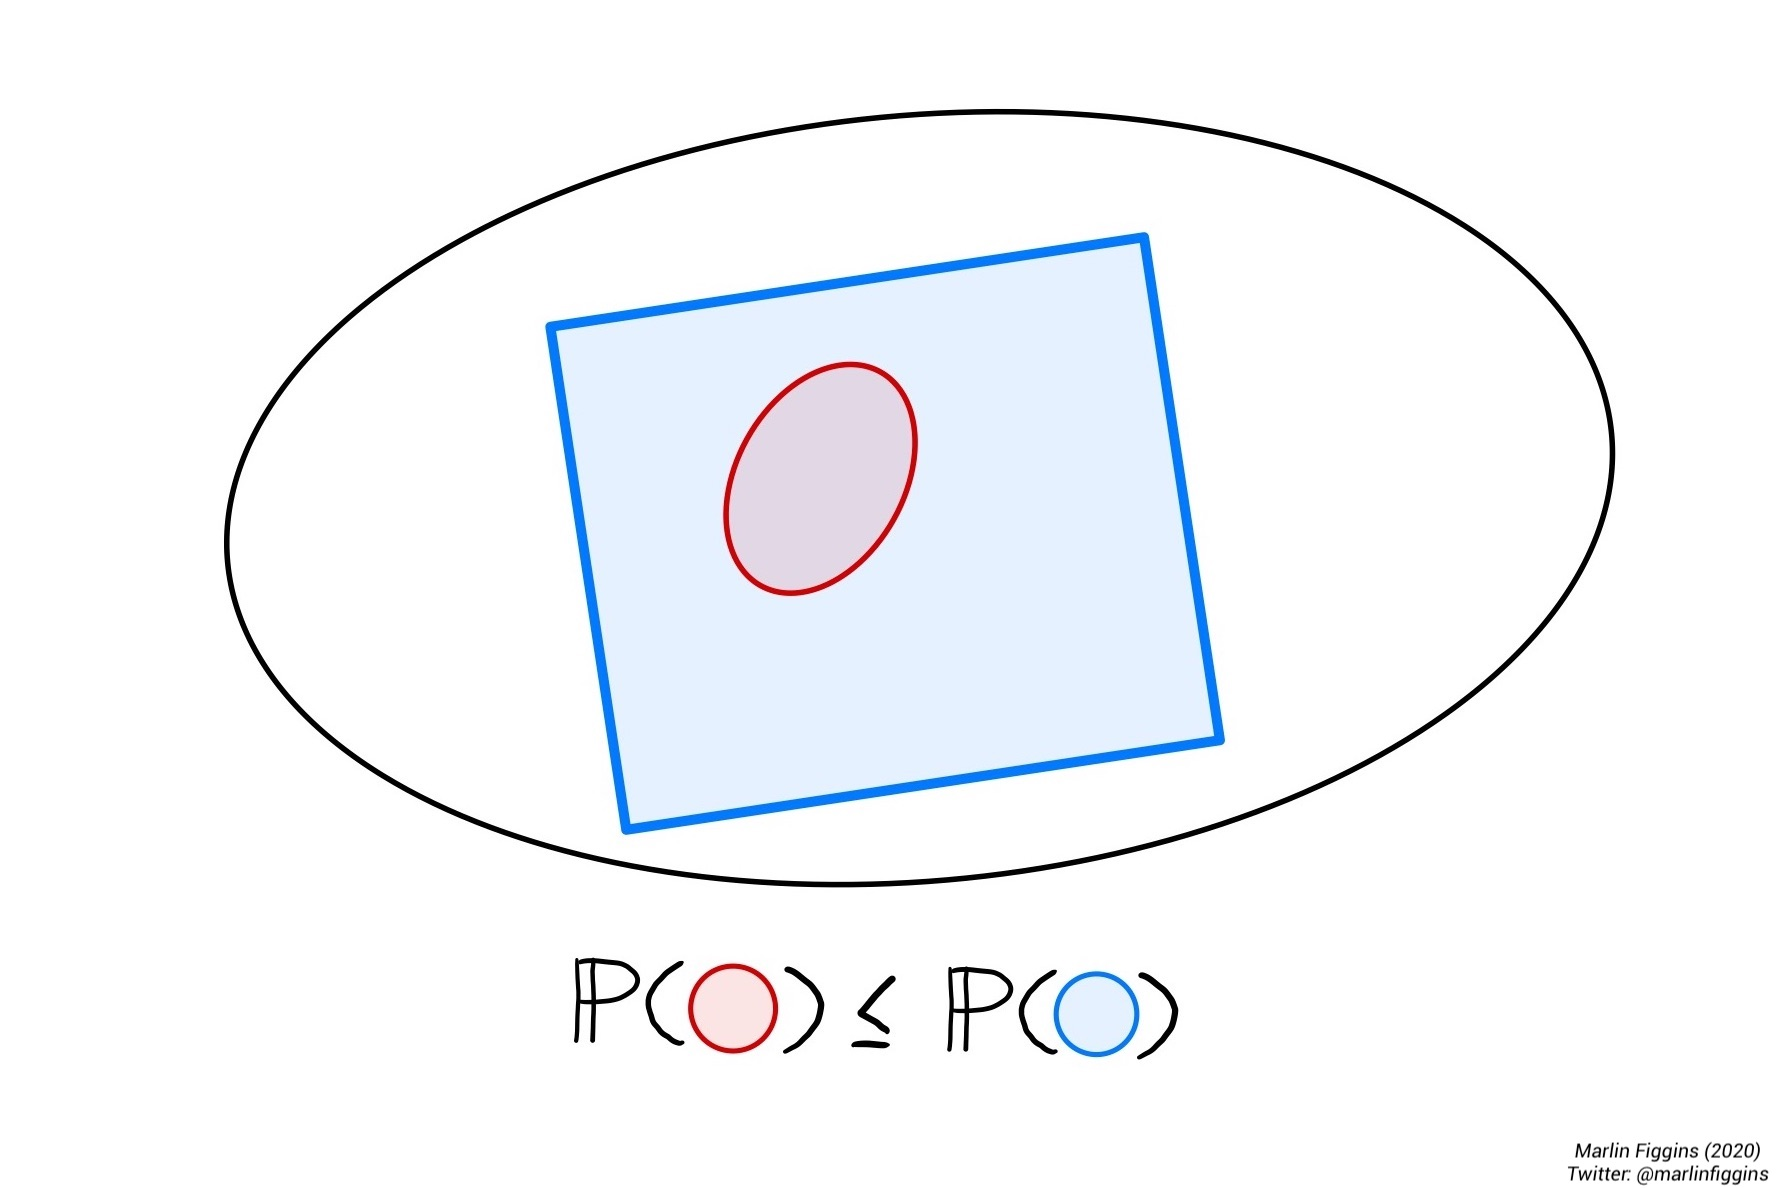
\includegraphics[width=0.6\linewidth]{intro-to-prob-subset-ineq.jpg}
   \caption{If a probability measure is consistent with our formulation, it ought to be monotonic. Appending additional outcomes to an event $E$ should never decrease its probability of occuring. }%
   \label{fig:intro-to-prob-subset-ineq}
 \end{figure}

 % TODO: Exposition about the fact that we can pass to limits
 \begin{thm}[Continuity of measure]\leavevmode
   \begin{enumerate}[(i)]
     \item \emph{Continuity from above.} If we have a sequence of increasing subsets $A_1 \subset A_2 \subset \cdots $ such that $\bigcup_i A_i = A$, then 
       \begin{equation}
         \mu(A_i) \uparrow \mu(A) \text{ as } i \to \infty.
       \end{equation}
     \item \emph{Continuity from below.} If we have a sequence of decreasing subsets $A_1 \supset A_2 \supset \cdots $ such that $\bigcup_i A_i = A$, then 
       \begin{equation}
         \mu(A_i) \downarrow \mu(A) \text{ as } i \to \infty. 
       \end{equation}
 \end{enumerate}
 \end{thm}

 \begin{exer}
   Prove that in a probability space $(\Omega, \calF, \Prob)$ 
   \begin{equation} 
     \Prob(A) = 1 - \Prob(A^c) \text{ for any event } A \in \cal F.
   \end{equation}
 \end{exer}

\subsection{Discrete Probability Spaces}%
\label{sub:discrete_probability_spaces}

\paragraph{Constructing a discrete probability space.}

We'll now focus on the case of discrete probability spaces. Let $\Omega$ be a countable set. That is, either finite or countably infinite. Also, let $\calF$ be the set of all subsets of $\Omega$ which we will call the power set $\mathcal{P}(\Omega)$. We can know endow $(\Omega, \calF)$ with a probability measure. 

\begin{thm}
  Suppose we have a countable set $\Omega$ with a $\sigma$-algebra $\calF=\mathcal{P}(\Omega)$. Then any function $p \colon \Omega \to [0, 1]$ such that 
\begin{equation}
  \sum_{\omega\in\Omega} p(\omega) = 1
\end{equation}
induces a probability measure $\Prob$ on $(\Omega, \calF)$ as follows. For any event $A\in \calF$, we define the probability of $A$ as 
\begin{equation}
  \Prob(A) = \sum_{\omega \in A} p(\omega).
\end{equation}
We call the function $p$ the \emph{probability mass function} of $\Prob$.
\end{thm}

\begin{exmp}[Repeated fair coins]
Consider the following experiment: We have a fair coin and we flip it until it lands on heads. We can write the possible outcomes as sequences of heads and tails, so that
\begin{equation}
  \Omega = \{ H, TH, TTH, TTH, \ldots \}.
\end{equation}

As before, we can let $\calF = \mathcal{P}(\Omega)$. Let's motivate our choice of probability mass function $p$. Assuming that the probability of heads and tails at every flip is $\frac{1}{2}$, then we have a probability of $\left(\frac{1}{2}\right)^n$ for having $n$ consequective flips. This tells us that
\begin{equation}
p(\underbrace{T\cdots T}_{n \text{ tails}} H) = \left(\frac{1}{2}\right)^n.
\end{equation}

We can check that this indeed sums to one:

\begin{equation}
  \sum_{\omega\in\Omega}p(\omega) = \sum_{i=1}^{\infty} \left(\frac{1}{2}\right)^n. 
\end{equation}

As shown above, this probability mass function induces a probability measure $\Prob$ on $(\Omega, \calF)$. We can now use this measure the compute the probability of events like:

\begin{align}
  A &= \{ \text{Heads appears before third toss.} \} = \{H, TH \},\\
  B &= \{ \text{There are an even number of tails.}\} = \{H, TTH, TTTTH, \ldots\}.
\end{align}

We can then compute these probabilities as:
\begin{align}
  \Prob(A) &= \frac{1}{2} + \frac{1}{4}, \\
  \Prob(B) &= \frac{1}{2} + \frac{1}{2^3} + \frac{1}{2^5} + \cdots = \frac{2}{3}.   
\end{align}
\end{exmp}

%TODO: Add text saying asking what would happen if we wanted to pass to ask about the long-term behavior of the coin-tossing experiment. What if we wanted to flip an infinite number of coins...

\subsection{Uncountable probability spaces}%
\label{sub:uncountable_probability_spaces}

%TODO: Add text stating that we can't simply use the the power set of uncountable sets to generate a $\sigma$-algebra.

We'll begin by further describing $\sigma$-algebra, so that we can understand what an uncountable $\sigma$-algebra must satisft. %TODO: Edit this slightly

\begin{prop}
  \emph{The intersection of $\sigma$-algebras is again a $\sigma$-algebra.} Let $I \neq \emptyset$ be an arbitrary set. If we have a collection of $\sigma$-algebras $\calF_i$ for $i\in I$ defined on $\Omega$, then their intersection 

  \begin{equation}
    \bigcap_{i\in I} \calF_i \text{ is a $\sigma$-algebra on } \Omega. 
  \end{equation}
\end{prop}

\begin{proof}
  Per an earlier exercise, all $\sigma$-algebras in the collection $\calF_i$ must contain $\emptyset$ and $\Omega$. Therefore, these sets are also in the intersection. For any event $A$ that is in every $\calF_i$, $A^c$ must be in $\calF_i$ since they are closed under complements. A similar argument holds for countable collections of events $A_j$ and their unions.
\end{proof}

Thus, if we are given a sample space $\Omega$ and $\mathcal{A}$ a collection of subsets of $\Omega$, then there is a smallest $\sigma$-algebra which contains $\mathcal{A}$. 

\begin{defn}[$\sigma$-algebra generated by $\mathcal{A}$]
  Given a sample space $\Omega$ and a collection of its subsets $\mathcal{A}$, the $\sigma$-algebra generated by $\cal{A}$ is the smallest $\sigma$-algebra containing $\mathcal{A}$. We denote this as $\sigma(\mathcal{A})$. 
\end{defn}

\begin{exmp}
  Given $\Omega = \{ 1,2,3,4 \}$ and $\mathcal{A} = \{ \{1\}. \{1,2\} \}$, the smallest $\sigma$-algebra containing $\mathcal{A}$ is
  \begin{equation}
    \sigma{\mathcal{A}} = \{\emptyset, \Omega, \{1\}, \{2,3,4\}, \{1,2\},\{3,4\},\{1,3,4\},\{2\}\}    
  \end{equation}
\end{exmp}

\paragraph{Constructing uncountable probability spaces}%
\label{par:constructing_uncountable_probability_spaces}

Let's consider the experiment of drawing a random number between $[0,1]$. In this case, our sample space is clearly $\Omega = [0,1]$. In this case, we would like each number to be equally likely, but we can't simply set each number to occur with probability $\Prob(A) = \frac{\abs{A}}{\abs{\Omega}}$ as with the case of the fair die because our space is uncountable! Ideally, we want to find some function $p(x)=p$ which describes the probability that we choose $x\in[0,1]$. What is the probabiltiy that our chosen number is rational (in $\bbQ$). By the countable additivity of our probability measure, 

\begin{align}
  \Prob(\bbQ \cap [0,1]) &= \Prob \left( \bigcup_{ x\in \bbQ\cap[0,1]} \{x\} \right) \\ 
                         &= \sum_{x\in Q\cap[0,1]} p(x) = \sum_{x\in Q\cap[0,1]} p. 
\end{align}

For any positive real value of $p$, the rightmost sum is infinite which is nonsensical as the probability of any event cannot exceed one. Thus the probability of an single value must be exactly 0. By the countable additivity of measure, this means that any countable subset of $[0,1]$ must have probablity 0.

\paragraph{The Lebesgue measure on $[0,1]$} We'll try an alternative approach to constructing probability spaces. We begin by defining the probabilities of certain subsets of interest and we extend this to the $\sigma$-algebra containing that collection of subsets. For example, we can specify that the probability of choosing a number between $a$ and $b$ is 

\begin{equation}
  \Prob((a,b]) = b - a \text{ for $a$ and $b$ with } 0\leq a < b \leq 1.
\end{equation}

This is a uniform probability measure on $[0,1]$ and it is called the \emph{Lebesgue measure on $[0,1]$}.

\paragraph{Borel $\sigma$-algebra}%
\label{par:borel_sigma_algebra}

We can extend the Lebesgue measure described below by extending it to the $\sigma$-algebra generated by intervals of the form $(a,b]$ by using the countable additivity property of measures. This is called the \emph{Borel $\sigma$-algebra} on $[0,1]$ is denoted by $\mathcal{B}([0,1])$. $\mathcal{B}([0,1])$ is the smallest $\sigma$-algebra containing all open sets in $[0,1]$. Additionally, the extension of our measure to the Borel $\sigma$-algebra is unique by the Caratheodory Extension theorem. That being said, the Lebesgue measure cannot be extended to all subsets of $[0,1]$. That being said, we will restrict our attention to study $([0,1], \mathcal{B}([0,1]))$. 

\begin{exmp}[Infinite coin tosses]
  Suppose that we conduct an infinite sequence of coin tosses. Let the probability of each coin showing heads be $p$ and the probability of tails be $q=1-p$. In this case, our sample space is all possible countable sequences of heads and tails. There is a one-to-one correspondence between $\Omega$ and $[0,1]$ by considering the base two expansion of numbers between $[0,1]$. As $\Omega$ is uncountable, we begin by specifying the probability on some reasonable subset of events which we can expand to some larger $\sigma$-algebra. We'll represent $w\in\Omega$ as a sequence $\omega_1\omega_2\ldots$ where each $w_i$ is the result of the $i$th coin toss. Let $A_H = \{ \omega\in\Omega\mid \omega_1 = H \}$.  That is, $A_H$ is the event that the first coin toss is heads. Naturally, the probability of $A_H$ should be the probability of flipping heads, so that

  \begin{equation}
    \Prob(A_H) = p \text{ and similarly } \Prob(A_T) = q = 1 - p.
  \end{equation}
  These events generate a $\sigma$-algebra $\calF_1 = \sigma(\{A_H, A_T \})$. In fact, we can define a series of $\sigma$-algebras $\calF_n$ based on the events of the first $n$ coin tosses. For example, consider $\calF_2$. This would contain events like:
\begin{align}
A_{HH} = \{\omega\in\Omega \mid \omega_1 = H, \omega_2 = H\}, &\quad A_{HT} = \{\omega\in\Omega \mid \omega_1 = H, \omega_2 = T\}, \\
A_{TH}= \{\omega\in\Omega \mid \omega_1 = T, \omega_2 = H\}, &\quad A_{TT}= \{\omega\in\Omega \mid \omega_1 = T, \omega_2 = T\}.
\end{align}

These events would have probabilities:
\begin{align}
  \Prob(A_{HH}) = p^2, &\quad \Prob(A_{HT}) = pq, \\
  \Prob(A_{TH}) = pq, &\quad \Prob(A_{TT}) = q^2.
\end{align}

We can similarly extend this to the events in $\calF_n$. Due to our construction, we have an increasing sequence of $\sigma$-algebras $\calF_1 \subset \calF_2 \subset \calF_3 \ldots$ which describe the results of finite coin tosses. We'll then define $\calF_\infty = \cup_{n\in\bbN} \calF_n$. This is \textbf{not} a $\sigma$-algebra because it is not closed under countable intersection. Consider the event $w_H$ which is the infinite sequence of outcomes with all $H$. We also consider the outcomes $\omega_{nH}$ which is where we count $n$ heads in a row. As you can see,
\begin{equation}  
  \{\omega_H \} = \bigcap_{n\in\bbN} \{\omega_{mH}\}.
\end{equation}
However,$ \{ w_H\}$ is not in $\calF_n$ for any $n$ since it depends on the results of all coin tosses. This means that $\calF_\infty$ cannot be a $\sigma$-algebra as it does not contain the countable union of $\{ \omega_{nH}\mid n\in\bbN\} \in \calF_\infty$. To remedy this, we can just use $\calF = \sigma(\calF_\infty)$. Once again, we can extend our probabilities to events in $\calF$ that are in $\calF_\infty$ uniquely. Unlike $\calF_\infty$, $\calF$ contains events which cannot be specified by any finite number of coin tosses like $\omega_H$ which we discussed before. We can assign a probability to this event using the continuity of measure from above. Since $\{\omega_{nH}\} \supset \{\omega_{(n+1)H}\}$ and $\{\omega_H \} = \cap_{n\in\bbN} \{\omega_{mH}\}$, it follows that 
\begin{equation}
  \Prob(\{\omega_{nH} \}) = p^n \downarrow \Prob(\{\omega_H\}) = 0.
\end{equation}
\end{exmp}

\subsection{Random variables and distributions}%
\label{sub:random_variables_and_distributions}

\paragraph{Defining random variables.}%
\label{par:defining_random_variables_}

Though probability spaces are plenty interesting themselves, we're often interested in evaluating functions of probability spaces to pick apart to answer the questions which interest us. For this purpose, we'll rely on random variables.

\begin{defn}
  Let $(\Omega, \calF, \Prob)$ be a probability space. A function $X\colon \Omega \to \bbR$ is called a random variable if for every Borel set $B\in \mathcal{B}(\bbR)$, we have that
  \begin{equation}
    X^{-1}(B) = \{ \omega \mid X(\omega) \in B\} \in \calF.
  \end{equation}
  To be precise about the choice of $\sigma$-algebra, we would say that $X$ is $\calF$-measurable and write $X \in \calF$.
\end{defn}

In the case where $\Omega$ is discrete, then any function $X\colon \Omega \to \bbR$ is a random variable because the $\sigma$-algebra $\calF = \mathcal{P}$ which contains all subsets of $\Omega$. 

\paragraph{Indicator functions}%
\label{par:indicator_functions}
 One of the most simple examples of random variables are the indicator function. An indicator function is a random variable of the form
 \begin{equation}
   \ind_A(\omega) = \begin{cases} 1, \quad \omega \in A \\
     0, \quad \omega \not\in A,
   \end{cases}
 \end{equation}
 where is some event $A\in\calF$. We can prove directly that $\ind_A$ is indeed a random variable through a bit of case work. Suppose that we have a Borel set $B$, then

 \begin{equation}
   \ind_A(B) = \begin{cases}
     A, \quad 1\in B \text{ and } 0 \notin B \\
     A^c, \quad 0 \in B \text{ and } 1\notin B \\
     \Omega, \quad 0,1 \in B \\
    \emptyset, \quad 0,1\not\in B.
   \end{cases}
 \end{equation}

\paragraph{Distributions of random variables.}%
\label{par:distributions}

We can use random variables to create entirely new probability distributions. 

\begin{prop}
  If $X$ is a random variable on $(\Omega, \calF, \Prob)$, then $X$ induces a new probability measure $\mu$ on $\bbR$ by
  \begin{equation}
    \mu(B) = \Prob(X \in B) = \Prob( X^{-1}(B) ).
  \end{equation}
\end{prop}
We call this new probablity measure the \emph{distribution of $X$.} We won't prove proposition entirely, but note that countable additivity follows from the fact that $\Prob$ is countably additive and 
\begin{equation}
   X^{-1}\left(\bigcup_{i\in\bbN} B_i\right) = \bigcup_{i\in\bbN} X^{-1}(B_i) 
\end{equation}
when the $B_i$ are disjoint.
%TODO: Rewrite this to say that proving that it is indeed a probability measure is an exercise.

\paragraph{Distributions functions}%
\label{par:distributions_functions}

The distribution of a random variable $X$ is usually described by its \emph{distribution function}
\begin{equation}
  F(x) = \Prob(X \leq x) = \Prob( X \in (-\infty, x) ).
\end{equation}

There are certain properties that distribution function must follow in order to properly characterize a probability distribution. 
\begin{prop}[Properties of distribution functions.]
  A distribution function $F$ must satisfy the following:\leavevmode
  \begin{enumerate}[(i)]
    \item $F$ must be non-decreasing.
    \item $F(x) \xrightarrow[x\to\infty]{} 1$ and $F(x) \xrightarrow[x\to-\infty]{} 0$.
    \item $F$ is right continuous i.e. $\lim_{y\to x^+}F(y) = F(x)$.
    \item If $F(x-) = \lim_{y\to x^-}F(y)$, then $F(x-)=\Prob(X<x)$.
    \item $\Prob(X = x) = F(x) - F(x-)$.
  \end{enumerate}
\end{prop}

\begin{proof}
  Insert proof.
\end{proof}
%TODO: Insert proof

%TODO: If a function has above properties it is the distribution of some random variable. Threorem and show sketch of the proof.
\begin{thm}
  If a function $F$ satisfies $(i), (ii)$, and $(iii)$ of the previous proposition, then it is the distribution function of some random variable,
\end{thm}
\begin{proof}[Sketch of proof]
  
\end{proof}

%TODO: Flesh out this section and reorganize.
\paragraph{Generating random variables}%
\label{par:generating_random_variables}

Though the distribution function may not actually have a proper incerse, we will call the random variable $X$ in the above theorem the inverse of $F$ and denote it as $F^{-1}$. Using the sketch outlined above, we can actually generate random variables using a bit of algebra and a computer. In computer systems, standard algorithms generate random variables with uniform distributions $U$. We can use this fact to find the proper inverse function taking $U$ to desired distribution of a random variable $X$
\begin{equation}
  F_X = F^{-1}(U).
\end{equation}

%TODO: Equality of distributions.

\paragraph{Density functions}%
\label{par:density_functions}

When the distribution function $F(x)$ of a random variable $X$ can be written in the form
\begin{equation}
  F(x) = \int_{-\infty}^{x} f(y)dy,
\end{equation}

we say that the random variable $X$ has density $f$. 
%TODO: The density must satisfy integral and non-negativity. Because of properties i, ii, blah blah, the density must satisfy...

%TODO: Uniform distributions on $[a, b]$
\begin{exmp}[Uniform distribution on $(a,b)$]
Suppose we're given a density function 
\begin{equation}
  f(x) = \begin{cases}
    \frac{1}{b-a}, \quad x\in[a,b] \\
    0, \quad \text{ otherwise.}
  \end{cases}
\end{equation}
Here $a$ and $b$ are real numbers such that $a<b$. We can integrate this function directly to find the distribution function of this random variable to find
\begin{equation}
  F(x) = \int_{-\infty}^{x} f(y)dy = \begin{cases}
    0, \quad x < a\\
    \frac{x}{b-a}, \quad a\leq x \leq b \\
    1, \quad x > b.
  \end{cases}
\end{equation}
This distribution is called the uniform distribution on $[a,b]$.
%TODO: Return to write shorthand for this distribution.
\end{exmp}

%TODO: Exponential distrbution with rate $\lambda$.
\begin{exmp}[Exponential distribution with rate parameter $\lambda$]
Suppose we're given the density funciton 
\begin{equation}
  f(x) = \begin{cases}
        \lambda e^{-\lambda x}, \quad x\geq 0\\
        0, \quad x < 0.
      \end{cases}
\end{equation}
Once again, we can integrate to find that 

\begin{equation}
  F(x)= \int_{-\infty}^{x}f(y)dy = \begin{cases}
        1 - e^{-\lambda x}, \quad x\geq 0\\
        0, \quad x < 0.
      \end{cases}
\end{equation}

This distribution is called the exponential distribution with rate parameter $\lambda$.
%TODO: Return to write shorthand for this distribution.
\end{exmp}

%TODO: Constructing the exponential function from Uniform. 
\paragraph{Constructing the exponential distribution}%
\label{par:constructing_the_exponential_distribution}

Following the sketch proof of INSERT REFERENCE, we can constuct an exponential random variable $X$ from the Uniform random variable on $[0,1]$. Starting with FORMULA REFERENCE
\begin{equation}
  X(\omega) = \sup\{y \mid F(y) > \omega \} = \sup\{ \omega \mid 1 - e^{\lambda y} < \omega \}.
\end{equation}

Since the distribution function is continuous, we can compute the above supremum as the value $x$ which satisfies $1 - e^{-\lambda x} = \omega$, Solving for $x$, we obtain that 
\begin{equation}
  X(\omega) = x = \frac{-\log(1-\omega)}{\lambda}.
\end{equation}

Therefore, if we wanted to generate random samples from an expoenetial random variable,, we could generate random numbers $\omega$ from the uniform distribution on $[0,1]$ and apply $X$ to them.

%TODO: What it means for a probability measure or distribution to be discrete. Quick mention of absolute continuity.

\paragraph{Discrete probability distributions}%
\label{par:discrete_probability_distributions}

A probability measure or distribution is called discrete if it only obtains positive value on a countable set.
%TODO: Give example of discrete distribution. Point masses.

%TODO: Point mass example

%TODO: Poisson example
% Another example of a discrete random variable is the Poisson distribution. 
\begin{exmp}[Poisson Random Variable]
  The Poisson random is a random variable defined on $\Omega = \{ 0, 1, 2 , \ldots \}$ with $\sigma$-algebra $\calF = \mathcal{P}(\Omega)$. It has probability mass function
  \begin{equation}
    \Prob(\omega = k) = \frac{\lambda^k}{k!} e^\lambda.
  \end{equation}
  %TODO: What is the Poisson used for?
\end{exmp}

\subsection{Expectation}%
\label{sub:expectation}

%TODO: We define the expectation as the Lebesgue Integral ,,,,

%TODO: Constructing the Lebesgue Integral. 1. Simple Functions. 2. Bounded Functions. 3. Non-negative Functions 4. General Functions.

\begin{defn}[Expectation of a random variable]
  The \emph{expctation of a random variable } $X\colon \Omega \to \bbR$ defined on a probability space $(\Omega, \calF, \Prob)$ is the Lebesgue integral
  \begin{equation}
    \Expect[X] = \int_\Omega X d\Prob.
  \end{equation}
\end{defn}

\paragraph{Computing expectations} Moving forward, we will show several examples and techniques which can be used to compute the expectation of random variables. 

\begin{exmp}[Expectation of an indicator function.]
The simplest case is that of indicator functions. Consider the indicator function $\ind_A$ for set $A\in\calF$. Fromt the definition of the expectation, we can write this as
\begin{equation}
  \Expect[ \ind_A ] = \int_\Omega \ind_A d\Prob = 1 \cdot \Prob(A) + 0 \cdot \Prob(A^c) = \Prob(A).
\end{equation}
This example shows that we can easily compute the expectation by treating the indicator function as a simple function, then computing the expectation accordingly.
\end{exmp}

The previous example gives some necessary insight to the kinds of tricks we'll have to use in order to compute some expectations, but there are some simplifications we can make based on our calculus intuition for computing the expectation for random variables. In the more general setting, we can use a change of variables to do this integration over the real numbers, so that the expectation of a random variable $X$ on $(\Omega, \calF, \Prob)$ is given by
\begin{equation}
  \Expect[X] = \int_\Omega X d\Prob = \int_\bbR x \Prob_X(dx),
\end{equation}
where $\Prob_X$ is the distribution of $X$ on $\bbR$. In the case $X$ is continuous and has a density function $f_X$, we have that 
\begin{equation}
  \Prob_X(dx) = f_X(x)dx.
\end{equation}
Therefore, the full expectation can be computed as 
\begin{equation}
  \Expect[X] = \int_\Omega X d\Prob = \int_\bbR x f_X(x) dx,
\end{equation}
for continuous random variables $X$ with density $f_X$.

When $X$ is instead discrete, then
\begin{equation}
  \Prob_X(dx) = \Prob(X^{-1}(\{x\})) = \Prob(X = x).
\end{equation}
This allows us to write the expectation as 
\begin{equation}
  \Expect[X] = \int_\Omega X d\Prob = \sum_{\omega\in\Omega} \omega \Prob(X = \omega).
\end{equation}

We can think of this as a change of variables from the probability space $(\Omega, \calF, \Prob)$ to the probability space $(\bbR, \mathcal{B}(\bbR), \Prob_X)$. 

Let's use this technique to compute the expectation of several of the random variables we've previously discussed. 

\begin{exmp}[Expectation of a Poisson Random Variable]
  Using the previous definition of the Poisson variable $X$ with rate parameter $\lambda$, we can compute the expectation as
  \begin{align}
    \Expect[X] = \int_\Omega X d\Prob = \sum_{k=0}^\infty k\Prob(X = k) = \lambda.
  \end{align}
\end{exmp}

\begin{exmp}[Expectation of an Exponential Random Variable]
  %TODO: ADD EXPOSITION
\begin{align}
  \Expect[X] = \int_\Omega X d\Prob = \int_\bbR x \lambda e^{-\lambda x}dx = \frac{1}{\lambda}.
\end{align}
\end{exmp}

We can also use this technique to compute the expectation of measurable functions $g$ of a random variable $X$. Since $g(X)$ itself is a random variable due to the measurability of $g$, we can compute the expecation of $g(X)$ as
\begin{equation}
  \Expect[g(X)] = \int_\Omega g(X)d\Prob = \int_\bbR g(x) \Prob_X(dx).
\end{equation}

This result allows us to prove some interesting consequences of the expectation. The most important one being that the expectation is linear.

\begin{thm}[Linearity of expectation]
  If $X$ and $Y$ are random variables and $a$ and $b$ are constants, then 
  \begin{equation}
    \Expect[aX + bY] = a \Expect[X] + b \Expect[Y].
  \end{equation}
\end{thm}

\section{Independence, Martingales, and Conditioning}%
  \label{sec:independence_martingales_and_conditioning}
  The following section will focus on describing independent events... There are several different ways of defining independence between the various objects we've studied, but the overarching idea is that....

  \subsection{Defining independence}%
  \label{sub:defining_independence}
  
  %TODO: Flesh this out. Discuss why independence is an interesting notion to be defined and why it is often simplifying.
  \paragraph{Independence of events}%
  \label{par:independence_of_events}
  
  Given a probability space, $(\Omega, \Prob, \calF)$, two events $A, B \in \calF$ are independent if $\Prob(A \cap B) = \Prob(A)\Prob(B)$.
 \begin{exmp}[Independence of coin tosses]
   Let's return to the example of infinite coin tosses. Consider the following two events 
   \begin{align}
     A_H = \{ \omega = H \} \quad A_{HH} \cup A_{TH} = \{ \omega_2 = H \}.
   \end{align}
   These two events are independent since $\Prob(A_H) = p$, $\Prob(A_{HH} \cup A_{TH}) = p^2 + qp = p$, and
   \begin{equation}
     \Prob(A_H \cap (A_{HH} \cap A_{TH})) = \Prob(A_{HH}) = p^2.
   \end{equation}
 \end{exmp} 

 \begin{prop}
 If events $A$ and $B$ are independent, then so are $A^c$ and $B$, $A$ and $B^c$, and $A^c$ and $B^c$.
 \end{prop}

 \begin{proof}
%TODO: Prove this as in lecture 5.
\end{proof} 

 \paragraph{Independence of random variables}%
 \label{par:independence_of_random_variables}
 Two random variables $X$ and $Y$ are independent if for all events $C, B \in \mathcal{B}$, 
 \begin{equation}
   \Prob(X \in C, Y \in D) = \Prob(X\in C)\Prob(Y \in D).
 \end{equation}
 
 %TODO: Give exposition for the following theorem

 \begin{thm}
Evens $A$ and $B$ are independent if and only their indicator random variables are independent.
 \end{thm}
\begin{proof}
  %TODO: Prove this as in lecture 5
\end{proof}
 \paragraph{Independence of $\sigma$-algebras}%
 \label{par:independence_of_sigma_algebras}
 
 Two $\sigma$-algebras $\mathcal{F}$ and $\mathcal{G}$ are independent if for all $A\in\mathcal{F}$ and $B\in\mathcal{G}$, the events $A$ and $B$ are independent. 

 %TODO: ADd that this means we're working in a larger sigma algebra and probability space which contains that sigma algebra

Going forward, we'll try to establish a relationship between the independence of random variables and $\sigma$-algebras. In order to do this, we first define the \emph{$\sigma$-algebra genereated by the random variable $X$} which we denote as $\sigma(X)$. 

\begin{defn}[$\sigma$-algebra generated by a random variable.]
  Given a random variable $X$ on the sample space $\Omega$, we define the collection of subsets of $\Omega$ of the form $\{X \in B mid B \in \mathcal{B}\}$ to be $\sigma(X)$. We call $\sigma(X)$ the \emph{$\sigma$-algebra genereated by the random variable $X$}.
\end{defn}

\begin{exmp}[Modeling stock prices]
  %TODO: Add the example from lecture 5.
\end{exmp}

%TODO: Finish this exposition.

Now that we have a notion of what are the possible events associated with a given random variable, we can define a notion of what information random variables need to be determined. That is, given a $\sigma$-algebra $\calF$, we say that the random variable $X$ is $\calF$-measurable if $\sigma(X)\subset \calF$. This means that the information of possible events defined in $\calF$ is sufficient in determining the value of the random variable $X$. The following theorem allows us to formally relate the independence of random variables with $\sigma$-algebras.

\begin{thm}\leavevmode
  \begin{enumerate}[(i)]
    \item If random variables $X$ and $Y$ are independent, then the $\sigma$-algebras generated by them are as well.
    \item Conversely, if two $\sigma$-algebras $\calF$ and $\mathcal{H}$ are independent with $X\in \calF$ and $Y\in\mathcal{G}$, then $X$ and $Y$ are independent.
  \end{enumerate}
\end{thm}
\begin{proof}
  %TODO: Proof from lecture 5.
\end{proof}

\paragraph{Independence of $n$ objects}%
\label{par:independence_of_n_objects}

We'll now extend our previous definitions of independence to work with finite collections of objects. First up are $\sigma$-algebras. We say that $\sigma$-algebras $\calF_1, \ldots, \calF_n$ are independent if whenever $A_i \in \calF_i$ for $i = 1, \ldots, n$, then 
\begin{equation}
  \Prob\left( \bigcap_{i=1}^{n} A_i \right) = \prod_{i=1}^n \Prob(A_i).
\end{equation}

Similarly, random variables $X_1, \ldots, X_n$ are independent if whenever $B_i\in\mathcal{B}$ for $i=1,\ldots,n$, then 
\begin{equation}
  \Prob\left( \bigcap_{i=1}^{n} \{X_i \in B_i \} \right) = \prod_{i=1}^n \Prob(X_i \in B_i). 
\end{equation}

Lastly, events $A_1, \ldots, A_n$ are independent if whenever $I\subset{1, \ldots, n}$, we have that 

\begin{equation}
  \Prob\left( \bigcap_{i\in I} A_i\right) = \prod_{i\in I} \Prob(A_i). 
\end{equation}
%TODO: Note about how this differs from the previous definitions.

These extensions also give us similar relationships between events and their indicator random variables.
\begin{prop}
If $A_1, \ldots, A_n$ are independent events, then $A_1^c, A_2, \ldots, A_n$ are independent and the indicator random variables for $A_1, \ldots, A_n$ are independent. 
\end{prop}

\paragraph{Pairwise independence vs independence}%
\label{par:pairwise_independence_vs_independence}

Events $A_1, \ldots, A_n$ for which 
\begin{equation}
  \Prob(A_i \cap A_j) = \Prob(A_i) \Prob(A_j), \quad i\neq j
\end{equation}
are called \emph{pairwise independent}. It is important to note the difference since all independent events are pairwise independent, but pairwise independent collections of events may not be independent.

\begin{exmp}[Pairwise Independent but not independent]
  %TODO: Example of pairwise independent events which are not independent. 

  Consider the random variables $X_1, X_2, X_3$ so that
  \begin{equation}
    \Prob(X_i = 0) = \Prob(X_i = 1) = \frac{1}{2}.
  \end{equation}
  Additionally, let's define the events $A_1 = \{X_2 = X_3\}, A_2 = \{X_1 = X_3\}, A_3 = \{X_1 = X_2\}$. These events are pairwise independent because for all $i\neq j$
  \begin{equation}
    \Prob(A_i \cap A_j) = \Prob( X_1 = X_2 = X_3 ) = \frac{1}{4} = \Prob(A_i)\Prob(A_j),
  \end{equation}
  but they cannot be independent because 
  \begin{equation}
    \Prob(A_1 \cap A_2 \cap A_3) = \Prob(X_1 = X_2 = X_3) = \frac{1}{4} \neq \Prob(A_1)\Prob(A_2)\Prob(A_3).
  \end{equation}
\end{exmp}

\paragraph{Independence of infinitely many objects}%
\label{par:independence_of_infinitely_many_objects}
%TODO: After the independece of finite collections.
%TODO: List possible items
We say that a infinite collection (of $\sigma$-algebras, random variables, or events) is independent if every finite subset of it is independent.

\subsection{Conditions for independence}%
\label{sub:conditions_for_independence}

Oftentimes, it is not easy to verify that two random variables are independent directly from the definition as that requires checking independence for every pair of Borel sets. In order to get around this, we'll discuss and develop an easier method for showing independence of random variables. We start by defining the joint distribution for pairs of random variables.

\begin{defn}[Joint distribution]
  The \emph{Joint distribution function} $F_{X,Y}: \bbR^2 \to [0,1]$ of two random variables $X$ and $Y$ defined on a probability space $(\Omega, \calF, \Prob)$ if given by 
\begin{equation}
  F_{X,Y}(x,y) = \Prob( X \leq x, Y \leq y).
\end{equation}
\end{defn}

As with our original definitions of the probability distribution function, we have special cases for jointly discrete and continuous random variables. We begin with the discrete case

\paragraph{Joint probability mass function}%
\label{par:joint_probability_mass}


  Two random variables are jointly discrete if the pair $(X,Y)$ takes values in a countable subset of $\bbR$. This allows us define a joint probability mass function as 
  \begin{equation}
  f_{X,T}(x_i, y_i) = \Prob(X = x_i, Y = y_i)
  \end{equation}

  \paragraph{Joint probabilty density function}%
  \label{par:joint_probabilty_density_function}
  
  We call a pair of random variables jointly continuous if their joint distribution function $F_{X,Y}$ can be written as 
  \begin{equation}
    F_{X,Y}(x,y) = \int_{-\infty}^x\int_{-\infty}^y f_{X,Y}(u,v)dvdu
  \end{equation}
  for some function $f_{X,Y}\colon \bbR^2 \to [0, \infty)$. We call this function the joint density function. This also means that we can write this density as
  \begin{equation}
    f_{X,Y}(x,y) = \frac{\partial^2}{\partial x \partial y}F_{X,Y}(x,y).
  \end{equation}

  In the cases where $(X,Y)$ are jointly discrete or continuous, it is pretty easy to compute $\Prob(X\in C, Y\in D)$ for Borel sets $C$ and $D$. We have either
  \begin{align}
    \text{Discrete: } \Prob(X\in C, Y\in D) &= \sum_{x_i \in C, y_j \in D} f_{X,Y}(x_i, y_j)\\
    \text{Continuous: } \Prob(X\in C, Y\in D) &= \int_C \int_D f_{X,Y}(x,y)dydx.
  \end{align}

  When we have a joint probability distribution, it is possible to recover the original distributions of its component random variables as follows
  \begin{equation}
    F_X(x) = \Prob(X\leq x) = \Prob(X \leq x, Y \leq \infty) = \lim\limits_{y\to\infty} F_{X,Y}(x,y).
  \end{equation}
  This distribution $F_X$ is called the marginal distribution function of $X$. This simplifies in the discrete and continuous cases in the predictable way.
  %TODO: Add align environemnt showing how this simplifies.

  The joint distribution function provides us with easy to check conditions for indepedence. 

  \begin{thm}
    Let $X$ and $Y$ be random variables defined on the probability space $(\Omega, \calF, \Prob)$. Then the following conditions are equivalent
    \begin{enumerate}[(i)]
      \item $X$ and $Y$ are independent
      \item $F_{X,Y}(x,y) = F_X(x)F_Y(y)$ for every $(x,y)\in\bbR^2$.
    \end{enumerate}
  Moreover, if the random variables are either jointly discrete or continuous we have that
  \begin{align}
    \text{Discrete: } f_{X,Y}(x, y) &= f_X(x)f_Y(y) \text{ for every } (x,y)\in\bbR^2\\
    \text{Continuous: } f_{X,Y}(x, y) &= f_X(x)f_Y(y) \text{ for almost every } (x,y)\in\bbR^2\\
  \end{align}
  \end{thm}
 \subsection{Variance and Covariance}%
 \label{sub:variance_and_covariance}

 The variance of a random variable $X$ is defined by
 \begin{equation}
   \Var[X] = \Expect[X-\Expect[X]]^2 = \Expect[X^2] - (\Expect [X])^2,
 \end{equation} 
 whenever this quantity is defined. The covariance of two random variables $X$ and $Y$ is defined by
 \begin{equation}
   \Cov[X,Y] = \Expect[ (X - \Expect[X])(Y - \Expect[Y]) ],
 \end{equation}
 whenever this quantity is defined. In a way, the covariance is a generalization of the variance since $\Cov[X,X] = \Var[X]$. Note that the variance is not a linear operator like the expectation. In fact, with a quick computation we can compute that for random variables $X,Y$ and constants $a,b\in\bbR$:
 \begin{equation}
   \Var[aX + bY] = a^2 \Var[X] + b^2 \Var[Y] + 2av\Cov[X,Y].
 \end{equation}

 In the special case that $\Cov[X,Y]=0$, we say that $X$ and $Y$ are uncorrelated. One quick observation is that independent random variables are uncorrelated. If $X$ and $Y$ are independent, then we have
 \begin{align}
   \Cov[X,Y] &= \Expect[ (X-\Expect X)(Y - \Expect Y) ]\\
             &= \Expect[ XY - \Expect X \cdot Y - X\cdot \Expect Y + \Expect X \Expect Y ]\\
             &= \Expect[XY] - \Expect[X]\Expect[Y] - \Expect[X]\Expect[Y] + \Expect[X]\Expect[Y]\\
             &= \Expect[XY] - \Expect[X]\Expect[Y] = 0.
 \end{align}
Though independent variables are uncorrelated, the converse is not true. Uncorrelated random variables are not necessarily indpendent.

%TODO: Example of uncorrelated non-independent r.v.s. CHeck lecture 6.

\begin{thm}
  Suppose $X$ and $Y$ are independent random variables with distributions $\mu$ and $\nu$. If $h:\bbR^2\to\bbR$ is a measurable function with $h\geq 0$ or $\Expect\abs{h(X,Y)}<\infty$, then
  \begin{equation}
    \Expect[ h(X,Y) ] = \int_{\bbR}\int_{\bbR} h(x,y)\mu(dx)\nu(dy).
  \end{equation}
  In particular, if $h(x,y) = f(x)g(x)$ which are measurable functions with $f,g\geq 0$ or $\Expect\abs{f(x)}$ and $\Expect\abs{g(x)}<\infty$, then
  \begin{equation}
    \Expect[f(X)g(Y)] = \Expect[f(X)]\Expect[g(Y)].
  \end{equation}
\end{thm}
A simple corollary of this fact is that if $X$ and $Y$ are independent, then $\Expect[XY] = \Expect[X]\Expect[Y]$.

\subsection{Sums of independent random variables}%
\label{sub:sums_of_independent_random_variables}

\begin{thm}
  If $X$ and $Y$ are independent with cummulative distribution functions $F_X = F$ and $F_G = G$, then
  \begin{equation}
    F_{X+Y} = \Prob(X + Y \leq z) = \int_\bbR F(z-y)dG(y).
  \end{equation}
  The integral on the righthand side is called the \emph{convolution of $F$ and $G$} and is denoted by $F*G$.
\end{thm}
\begin{proof}
  Let $h(x,y) = \ind_{ \{x+y\leq z\} }$ and $\mu$ and $\nu$ bwe the probability measures with distributions $F$ and $G$. Then using the previous theorem, we have that
\begin{equation}
    \Expect[ h(X,Y) ] = \int_{\bbR}\int_{\bbR} h(x,y)\mu(dx)\nu(dy).
\end{equation}
Subbing in our choice of $h$, we see that
\begin{equation}
  \Expect[ h(X,Y) ] = \Expect \ind_{ \{X+Y \leq z\} } = \Prob(X + Y \leq z).
\end{equation}

On the other hand, we can simply the integral $\int_\bbR h(x,y) \mu(dx)$ as 
\begin{align}
  \int_\bbR h(x,y) \mu(dx) &= \int_\bbR \ind_{\{x+y \leq z \}} \mu(dx)\\
                           &= \int_bbR \ind_{\{x\leq z-y\}} \mu(dx)\\
                           &= \Prob(X \leq z-y) = F(z-y).
\end{align}
Putting these substitutions together, we get that
\begin{equation} 
  F_{X+Y} = \Prob(X + Y \leq z) = \int_\bbR F(z-y)\nu(dy) = \int_\bbR F(z-y)dG(y).
\end{equation}
\end{proof}

We'll use a special case of this theorem for when $X$ and $Y$ have density functions to give a more concrete example.
\begin{thm}
Suppose that we have two indepedent random variables $X$ with distribution $F$ and density $f$ and $Y$ has distribution $G$ . Then $X+Y$ has density
\begin{equation}
  f_{X+Y}(z)= \int_\bbR f(z-y)dG(y).
\end{equation}
When $Y$ additionally has density $g$, the last formula can be written as 
\begin{equation}
  f_{X+Y}(z)= \int_\bbR f(z-y)g(y)dy. 
\end{equation}
\end{thm}

%TODO: Proof with change of variables and Fubini's

\begin{defn}[Gamma distribution with parameters $\alpha$ and $\lambda$]
  %TODO: Add more about this RV
  The gamma density with parameters $\alpha$ and $\lambda$ is given by
  \begin{equation}
    f(x) = \begin{cases}
      \lambda^\alpha x^{\alpha-1}e^{-\lambda x} / \Gamma(\alpha), \quad& x\geq0\\
      0, \quad& x<0
    \end{cases}
  \end{equation}
where $\Gamma(\alpha) = \int_0^\infty x^{\alpha - 1}e^{-x}dx.$ If a random variable $X$ has density as above, we say that $X$ is gamma distributed and write $X\sim\text{Gamma}(\alpha, \lambda)$
\end{defn}


\begin{prop}[Sum of independent Gamma-distributed random variables.]
  If $X$ and $Y$ are two independent random variables with densities $\text{Gamma}(\alpha, \lambda)$ and $\text{Gamma}(\beta, \lambda)$, then $X+Y$ has gamma density with parameters $\alpha + \beta$ and $\lambda$.
\end{prop}
%TODO: Do proof which is a computation in Lecture 7.

A basic corollary of this is that if $X_1, \ldots, X_n$ are independent exponential random variables with parameter $\lambda$, then $X_1 + \cdots + X_n$ has a $\text{Gamma}(n, \lambda)$ distribution. 
%TODO: Make this a proposition

\begin{proof}
  An exponential distribution with rate parameter $\lambda$ is simply a gamma distribution with parameters $1$ and $\lambda$.
\end{proof}

\begin{defn}[Normal random variable with mean $\mu$ and variance $\sigma^2$]
  A normal random variable with mean $\mu$ and variance $\sigma^2$ has density
  \begin{equation}
    f(x) = \frac{1}{\sqrt{2\pi \sigma^2}} e^{-\frac{(x-\mu)^2}{2\sigma^2}}.
  \end{equation}
  If $X$ has density as above, we say that $X$ is an normal with mean $\mu$ and variance $\sigma^2$ and write $X\sim \text{Normal}(\mu, \sigma^2)$.
\end{defn}

\begin{thm}
  IF $X\sim \text{Normal}(\mu, a)$ and $Y\sim \text{Normal}(\nu, b)$ are two independent normal random variables, then $X+Y$ is normal with mean $\mu + \nu$ and variance $a+b$.
\end{thm}

%TODO: Be consistent with the ~. notation throughout

\begin{proof}
  %TODO: Proof
\end{proof}

\subsection{Conditional Expectation}%
\label{sub:conditional_expectation}

Given a probability space $(\Omega, \calF_0, \Prob)$ a sigma-algebra $\calF\subset\calF_0$ and a random variable $X\in\calF_0$ with $\Expect\abs{X}<\infty$. WE define the conditional expectation of $X$ given $\calF$ is any random variable $\Expect(X\mid\calF)$ which statisfies 
\begin{enumerate}[(i)]
  \item $\Expect(X\mid\calF)$ is $\calF$-measurable
  \item for all events $A\in\calF$, $\int_A X d\Prob = \int_A Yd\Prob$.
\end{enumerate}
 Any random variable satisfying the above two conditions is a version of the conditional expectation. The first thing we will settle is that this always exists and is unique. 

\begin{proof}[Proof of uniqueness]
  Suppose there are two random variables which satisfy $A_\epsilon = \{\omega \mid Y(\omega)-Y'(\omega)\geq \epsilon > 0 \}$, then 
  \begin{align}
    0 = \int_{A_\epsilon} (X - X)d\Prob = \int_{A_\epsilon} (Y - Y')d\Prob \geq \epsilon \int_{A_\epsilon}d\Prob = \epsilon \Prob(A_\epsilon),
  \end{align}
  so $\Prob(A_\epsilon)$. Since this holds for $\epsilon >0$, we have $Y\leq Y'$ almost surely. Similarly, interchanging $Y$ and $Y'$, we see that $Y = Y'$ almost surely.

  \paragraph{Examples of conditional expectation}%
  \label{par:examples_of_conditional_expectation}
 
  \begin{exmp}[Perfect Information]
  \end{exmp}

  \begin{exmp}[No information]
  \end{exmp}

  In the previous two examples, we've played a game of guess and check. Going forward, we'll relate this notion to conditional expectation to the one usually taught in undergrad probability.

  \begin{exmp}[Partitioning $\Omega$.]
  \end{exmp}

  \paragraph{Conditional Expectation of events}%
  \label{par:conditional_expectation_of_events}
  
\paragraph{Conditioning with respect to random variables}%
\label{par:conditioning_with_respect_to_random_variables}


  
\end{proof}
  \section{Characteristic Functions}%
  \label{sec:characteristic_functions}
  
  \section{Markov Chains}%
  \label{sec:markov_chains}
  
  \section{Generating Functions and Branching Processes}%
  \label{sec:generating_functions_and_branching_processes}
  
  \section{Convergence of Random Variables}%
  \label{sec:convergence_of_random_variables} 

\end{document}
